\documentclass{article}
% basics
\usepackage{amsfonts}
\usepackage{enumitem}
\usepackage{float}
\usepackage{graphicx}
\usepackage{hyperref} 
\usepackage[labelfont=bf]{caption}

\newtheorem{theorem}{Theorem}
\newtheorem{lemma}[theorem]{Lemma}
\newtheorem{corollary}{Corollary}[theorem]

% unique math expressions:
\usepackage{amsmath}
\DeclareMathOperator*{\andloop}{\wedge}
\DeclareMathOperator*{\pr}{Pr}
\DeclareMathOperator*{\approach}{\longrightarrow}
\DeclareMathOperator*{\eq}{=}

% grey paper
\usepackage{xcolor}
% \pagecolor[rgb]{0.11,0.11,0.11}
% \color{white}

% embedded code sections
\usepackage{listings}
\definecolor{codegreen}{rgb}{0,0.6,0}
\definecolor{codegray}{rgb}{0.5,0.5,0.5}
\definecolor{codepurple}{rgb}{0.58,0,0.82}
\lstdefinestyle{mystyle}{
    commentstyle=\color{codegreen},
    keywordstyle=\color{magenta},
    numberstyle=\tiny\color{codegray},
    stringstyle=\color{codepurple},
    basicstyle=\ttfamily\footnotesize,
    breakatwhitespace=false,         
    breaklines=true,                 
    captionpos=b,                    
    keepspaces=true,                 
    numbers=left,                    
    numbersep=5pt,                  
    showspaces=false,                
    showstringspaces=false,
    showtabs=false,                  
    tabsize=2
}

\lstset{style=mystyle}

\begin{document}
\author{Yosef Goren - Or Rubin}
\title{Graph Separation - Final Report}
\maketitle
\part*{Abstract}
The problem of graph separation is a well known problem in graph theory and has many applications.
There are currently no known algorithms that solve the problem accurately in polynomial time, and it is an open
problem whether the class of isomorphic graphs is NP-complete.\\
In this report, we applied the GIN network presented by Xu [2] to find a partial solution to this problem, 
similarly to the 1-WL test.


\part*{Introduction}
In the theory of message passing networks (MPNs); a well known result states 
that in the context of graph separation - the expressive of the MPNs is equal to the 1-WL isomorphism test.
More accurately, MPNs is a general framework for graph neural networks that can be
instantiated in many ways. While any realization of an MPN cannot separate
graphs unless they are separable by the WL isomorphism test, the converse
claim can be showed to be true for specific MPN constructions. The two classical
constructions of MPNs which are equivalent to WL are by Xu [2] and by
Morris [1].\\

A key result for the proof of separation of GINs in Lemma 5. The lemma
states that if $\mathcal{X}$ is a countable set and N is a fixed natural number, there
A key result for the proof of separation of GINs in Lemma 5. The lemma
states that if $\mathcal{X}$ is a countable set and N is a fixed natural number, there
exists a function $f : \mathcal{X} \rightarrow R$ such that, for every $X_1, X_2 \subseteq \mathcal{X}$
of size $<$ N,
\[
    \sum_{x\in X_1}f(x) \neq \sum_{x\in X_2}f(x)
\]

In GINs, this $f$ is replaced with an MLP m which can approximate $f$
arbitrarily well due to the universality of MLP. Note however that it is
not clear how large the MLP must be in order to be a good approximation
of $f$ . In fact, we will show that an MLP of fixed size can never enjoy the
same separation properties that f has. For simplicity we will focus on
univariate functions.

\begin{lemma}
    Let $\mathcal{X}=\mathbb{Z}$, $m:\mathbb{R}\to\mathbb{R}$ is a continuous piecewise linear function,
    then there exist multi-sets $X_1 \neq X_2 \subseteq \mathcal{X}$ such that \\
    \[ \sum_{x\in X_1}m(x) \neq \sum_{x\in X_2}m(x) \]

\end{lemma}
$Proof:$ \\
Since there are a finite amount of linear segments to it,
and the input range is infinite, there must be at-least
one segment which is infinitly long: in particular,
there must be a segment $[x_1,x_1+4], x_1\in\mathbb{Z}$
where $m$ corresponds to some affine function.\\
If we denote $y_1=m(x_1), y_2=m(x_1+4), s = \frac{y_2-y_1}{4}$.\\
We can find that affine function as:
\[
    \forall x\in \{x_1+i\mid i\in[3]\}, m(x)=s\cdot x+y_1
\]
Denote $X_1=\{x_1,x_1+4\}, X_2=\{x_1+1,x_1+3\}$.
Now we can see that:
\[
    \sum_{x\in X_1}m(x)=
    (2x_1+4)s+2y_1=
    \sum_{x\in X_2}m(x)
\]



\begin{corollary}
For any affine function $m(x) = ax + b $ there exists finite sub-multisets $X_1 \neq X_2 \subseteq \mathcal{X}$ such that

\[ \sum_{x\in X_1}f(x) \neq \sum_{x\in X_2}f(x) \]
\end{corollary}
\begin{corollary}
Since the MLP in the GIN uses a ReLU activation functions, as explained by Hanin \cite{Hanin}, the MLP is a piecewise linear function. 
Thus, if the GIN uses a pooling layer is piecewise linear, as maximum or, then the GIN network represent a piecewise linear function.
\end{corollary}



\part*{Methods}
\section*{Metrics}
To determine the quality of separation yielded by the model, we have considered a few metrics.\\
Note that we are using a finite size of $\mathcal{X}$ in these tests. Hence, $\mathcal{X}$
is also a finite set in the definitions of these metrics (the metrics are a function of both the model and the test sample).
\begin{itemize}
    \item Given a model $M:\mathcal{X}\rightarrow\mathbb{R}$, 
    we will look at $M^{-1}:\mathbb{R}\rightarrow\mathcal{X}$ s.t. 
    $\forall r\in\mathbb{R}, M^{-1}(r)=\{x\in\mathcal{X}:M(x)=r\}$.

    The first metric is calculated as follows:
    \[
        \frac{\sum_{r\in\mathbb{R}\wedge |M^{-1}(r)|>1}|M^{-1}(r)|}
        {|\mathcal{X}|}
    \]

    This metric is the proportion between the number of elements 
    that are collided and the total number of elements in the test set.
    
    We will refer to this as the 'count metric'.

    \item The second metric is the probability of collision
    between two uniformly sampled samples from the test set.
    This metric can be calculated as follows:

    \[
        \frac{\sum_{r\in\mathbb{R}\wedge M^{-1}(r)\neq\emptyset}|M^{-1}(r)|\cdot\left(|M^{-1}(r)|-1\right)}
        {|\mathcal{X}|\cdot\left(|\mathcal{X}|-1\right)}
    \]

    We will refer to this metric as the 'probability metric'.
\end{itemize}


\section*{Training}
Since we aim to pervert collisions, an intuitive hubristic at achieving this would be to keep
outputs as distant as possible.
Hence, we suggest the loss to be the negative distance between the outputs of the model:
\[
    L(G_1,G_2)=-|M(G_1)-M(G_2)|    
\]

The actual training process for out GIN model, was done the same way as seen in  Xu [2].

\section*{Dataset}
To create our dataset we are randomly generating Erdos-Renyi graphs using the networkx library. The edge probabilities of
these graphs is a parameter of the dataset. An additional parameter of the detaset is ofcourse is the number
of nodes in each graph. We later test the effect of these parameters on the model's performance.\\

\part*{Experiments}
\subsection*{Parameters Effects on Untrained Models}
The parameters have tested are the number of nodes in the graphs ,the edge probability and an additional parameter
relates to the depth and width of neural network inside the GIN model; we call this parameter the 'network size'.
The network size parameter dictates both the depth and width of the neural network inside the GIN model in the following manner:
\begin{itemize}
    \item The depth of the neural network is the same as the 'network size' parameter.
    \item The width of the neural network is 32 times the 'network size' parameter.
\end{itemize}
Indeed these restrictions over the network seem quite arbitrary but we believe that while performance might be maximaized by
a different set of restrictions, we will still be able to see the effect of the parameters on the model's performance with these restrictions.\\
In order to estimate the effects of different parameters, we have applied grid sampling of the parameters.
Each point in this grid was sampled with a set of 200 graphs.
For each parameter value we show the average of the results over the rest of the configurable parameters.

In figures 1 to 6 we can see the effect of each parameter on each of the metrics we have defined.
The figures 1-3 relate to the collision count metric while figures 4-6 relate to the collision probability metric.
We can see that an increase occurs In figures 1 and 4 we can see that the more edges we have - the more collisions we have.
In figures 2 and 5 we see that the metrics values peek when the 'network size' is at 5,
while the decrease in values grater than 5 are not dramatic.
In figures 3 and 6 we see that the relation between the edge probability and the metrics is almost linear where the
higher the edge probability - the higher are the metric values.

\begin{figure}
    \begin{center}
        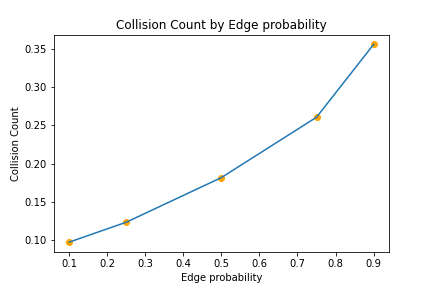
\includegraphics[width=7cm]{../figures/Collision_Count_edge_prob.png}\\
        \caption{The effect of probability for the existence of an edge between two nodes on the model's collision count metric.}
    \end{center}
\end{figure}    
\begin{figure}
    \begin{center}
        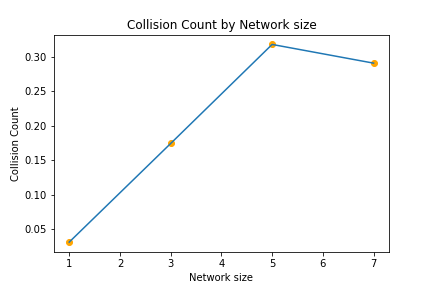
\includegraphics[width=7cm]{../figures/Collision_Count_network_size.png}\\
        \caption{The effect of the size of model's network on the model's collision count metric.}
    \end{center}
\end{figure}    
\begin{figure}
    \begin{center}
        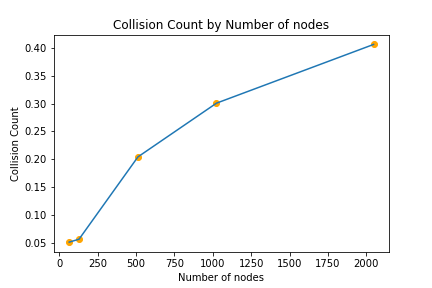
\includegraphics[width=7cm]{../figures/Collision_Count_num_nodes.png}\\
        \caption{The effect of the number of nodes on the model's collision count metric.}
    \end{center}
\end{figure}    
\begin{figure}
    \begin{center}
        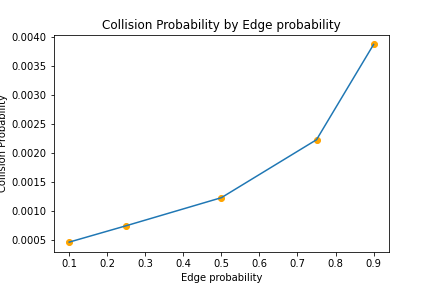
\includegraphics[width=7cm]{../figures/Collision_Probability_edge_prob.png}\\
        \caption{The effect of probability for the existence of an edge between two nodes on the model's collision probability metric.}
    \end{center}
\end{figure}    
\begin{figure}
    \begin{center}
        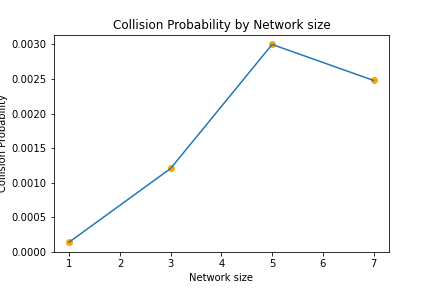
\includegraphics[width=7cm]{../figures/Collision_Probability_network_size.png}\\
        \caption{The effect of the size of model's network on the model's collision probability metric.}
    \end{center}
\end{figure}    
\begin{figure}
    \begin{center}
        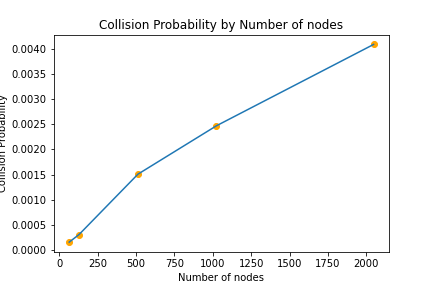
\includegraphics[width=7cm]{../figures/Collision_Probability_num_nodes.png}\\
        \caption{The effect of the number of nodes on the model's collision probability metric.}
    \end{center}
\end{figure}    

\subsection*{Training Effect}
In this experiment, we set a parameter configuration and compare the model results between an untrained GIN model
and the trained GIN model over a test set.
As one can see, in figure 7, training the models had a
meaningful effect on the model's performance in graph separation; as measured by our metrics.
\begin{figure}
    \begin{center}
        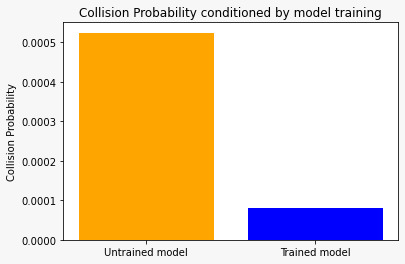
\includegraphics[width=7cm]{../figures/Training_Performance_Bars.png}\\
        \caption{The effect of training the network on the model's collision probability metric.
        These results were taken from a test set of 10,000 graphs.}
    \end{center}
\end{figure}    


\part*{Conclusion}
We can see that the both the node count and the edge probability parameter increase both metrics (meaning we get more collisions),
while the network size parameter has a more complex effect on the metrics: smaller networks seem to be more capable of graph sepration
when they are not trained.\\
We can see that GIN's are capable of separating graphs, and that these results can be further improved by training.
Even after training, the separation is not perfect, and we can see that the model still yields collisions.


\part*{Future Work}
As we have mentioned before, we still might want to try and get better separation using these GIN models,
and we suspect there might be other loss functions which will enable training the models to better suit
the metrics which we have defined. For example, the current loss function does not drop off it's value
as the distance between the outputs of the model increases. This might be a problem, since we
only care if the outputs are far enough apart, and not how far they are apart. Hence a we suggest trying to
apply these experiments with a loss function which drops off as the distance between the outputs increases.\\
Another interesting work that might be relevant here, would be to compare the results of the GIN model to
the 1-WL test over the same datasets used here. In theory, the 1-WL test should have an equivalent expressive power as
the GIN model.\\
Additionally, it might be interesting to try these models out on 'real' datasets,
rather than the synthetic ones we have used here. \\
In the conclusions we have mentioned that - perhaps surprisingly - smaller neural networks have yielded function with better separation ability when not trained,
an interesting followup might be to see why this is the case, and check whether this is any different when the models are trained.
Finally, we might want to reconsider the restrictions we have placed on the network size parameter - and consider different option
in an attempt to maximized the GINs performance.

\begin{thebibliography}{9}
    \bibitem{Morris}
    Morris, D. (2019). Message Passing Neural Networks. arXiv preprint arXiv:1910.00825.
    \bibitem{Xu}
    Xu, K., Li, W., \& Leskovec, J. (2019). How Powerful are Graph Neural Networks?. arXiv preprint arXiv:1810.00826.
    \bibitem{Hanin}
    Hanin, B., \& Rolnick, D. (2019). Complexity of Linear Regions in Deep Networks. ArXiv:1901.09021
\end{thebibliography}
\end{document}